%!TEX root = ../documentation.tex


\chapter{Anbindung externer Dienste - Dropbox}

Eines der Ziele von Norbert - Your StudyBuddy ist es Wissensmanagement zu betreiben und somit Wissen zu sammeln und weiterzugeben. Da Informationen und Wissen von Studierenden einer DHBW meistens in Dropbox abgelegt werden, wird in diesem Kapitel die Anbindung von Dropbox an Norbert beschrieben. Dabei wird zunächst erst allgemein auf den standardisierten Autorisiuerngsprozess \enquote{OAuth} eingegangen und daraufhin die verschiedenen Dropbox Endpoints mit ihren Schnittstellen vorgestellt.


\section{Autorisierungsprozess (OAuth)}

OAuth ist ein offenes Protokoll, dass eine standardisierte und sichere API-Autorisierung für mobile Endgeräte, Webanwendungen und Desktop-Applikationen ermöglicht. Der Benutzer kann über den OAuth-Autorisierungsprozess (Abbildung \ref{04ergebnis:oauth}) einer Anwendung (in diesem Fall Norbert) Zugriff auf gespeicherte Daten erlauben. Dabei loggt sich der Benutzer über die Applikation (Norbert) die Zugriff benötigt auf dem Dienst, der die freizugebenden Daten speichert, ein (hier Dropbox) und erlaubt somit der Applikation den Zugriff. Dabei wird ein spezieller App key mit entsprechendem App scecret und ein Access-Token zwischen der Applikation und dem Dienst ausgetauscht. Der Access-Token wird individuelle für jeden Benutzer erstellt und wird bei API-Aufrufen mitgesendet. Dieser dient somit zur Authentifizierung des Benutzers, sodass kein Benutzername oder Passwörter ausgetauscht oder gespeichert werden müssen.

\begin{figure}[H]
\centering
	\scalebox{0.5}{\input{uml-diagramms/oauth}}
	\caption{OAuth-Autorisierungsprozess zwischen Norbert und Dropbox.com}
	\label{04ergebnis:oauth}	
\end{figure}


\section{Dropbox Endpoints}

Die Dropbox API besteht aus mehreren Endpoints (Abbildung \ref{04ergebnis:dpendpoints}), die jeweils unterschiedliche Funktionene bereitstellen. Alle API-Aufrufe benötigen zu Autorisierung den individuellen Access-Token eines Benutzers.

\begin{enumerate}
	\item \textit{dropbox.com:} Über diesen Endpoint/Webseite wird die OAuth-Autorisierung durchgeführt. Es wird nur einmalig zur Generierung des Access-Tokens ein Kontakt zu diesem Endpoint hergestellt.
	
	\item \textit{api.dropboxapi.com (RPC-Endpoint):}  Über die Domain api.dropboxapi.com können RPCs (remote procedure calls) ausgeführt werden. Dabei nimmt dieser Endpoint JSON-Strings im HTTP-Body entgegen und führt je nach aufgerufener URL verschiedene Funktionen aus. Ein RPC-Funktion ist beispielsweise list\_{folder} (\textit{https://api.dropboxapi.com/2/files/list\_{folder}}), die als Parameter einen Pfad erwartet und dann alle im entsprechenden Ordner sich
 befindenden Dateien auflistet. Das Ergebnis der Funktion wird daraufhin wieder im JSON-Format zurückgesendet.
 
 	\item \textit{content.dropboxapi.com (Download/Upload-Endpoint):} Wie der Name schon sagt, können über den Download/Upload-Endpoint Dateien heruntergeladen werden oder hochgeladen werden. Die benötigten Meta-Daten (Pfad, Datei ID etc.) werden dabei im HTTP-Header als JSON oder URL-Argument übergeben. Funktionsergebnisse werden im JSON-Format im HTTP-Response Header übergeben und Dateien im HTTP-Body übersendet.
\end{enumerate}

\begin{figure}[H]
\centering
	\scalebox{0.5}{% Graphic for TeX using PGF
% Title: C:\Users\Philipp Pütz\Desktop\Vorlesung - Software Engineering I\norbert\dokumentationen\softwareentwurf\uml-diagramms\dropboxendpoints.dia
% Creator: Dia v0.97.2
% CreationDate: Sun Mar 27 17:07:30 2016
% For: Philipp Pütz
% \usepackage{tikz}
% The following commands are not supported in PSTricks at present
% We define them conditionally, so when they are implemented,
% this pgf file will use them.
\ifx\du\undefined
  \newlength{\du}
\fi
\setlength{\du}{15\unitlength}
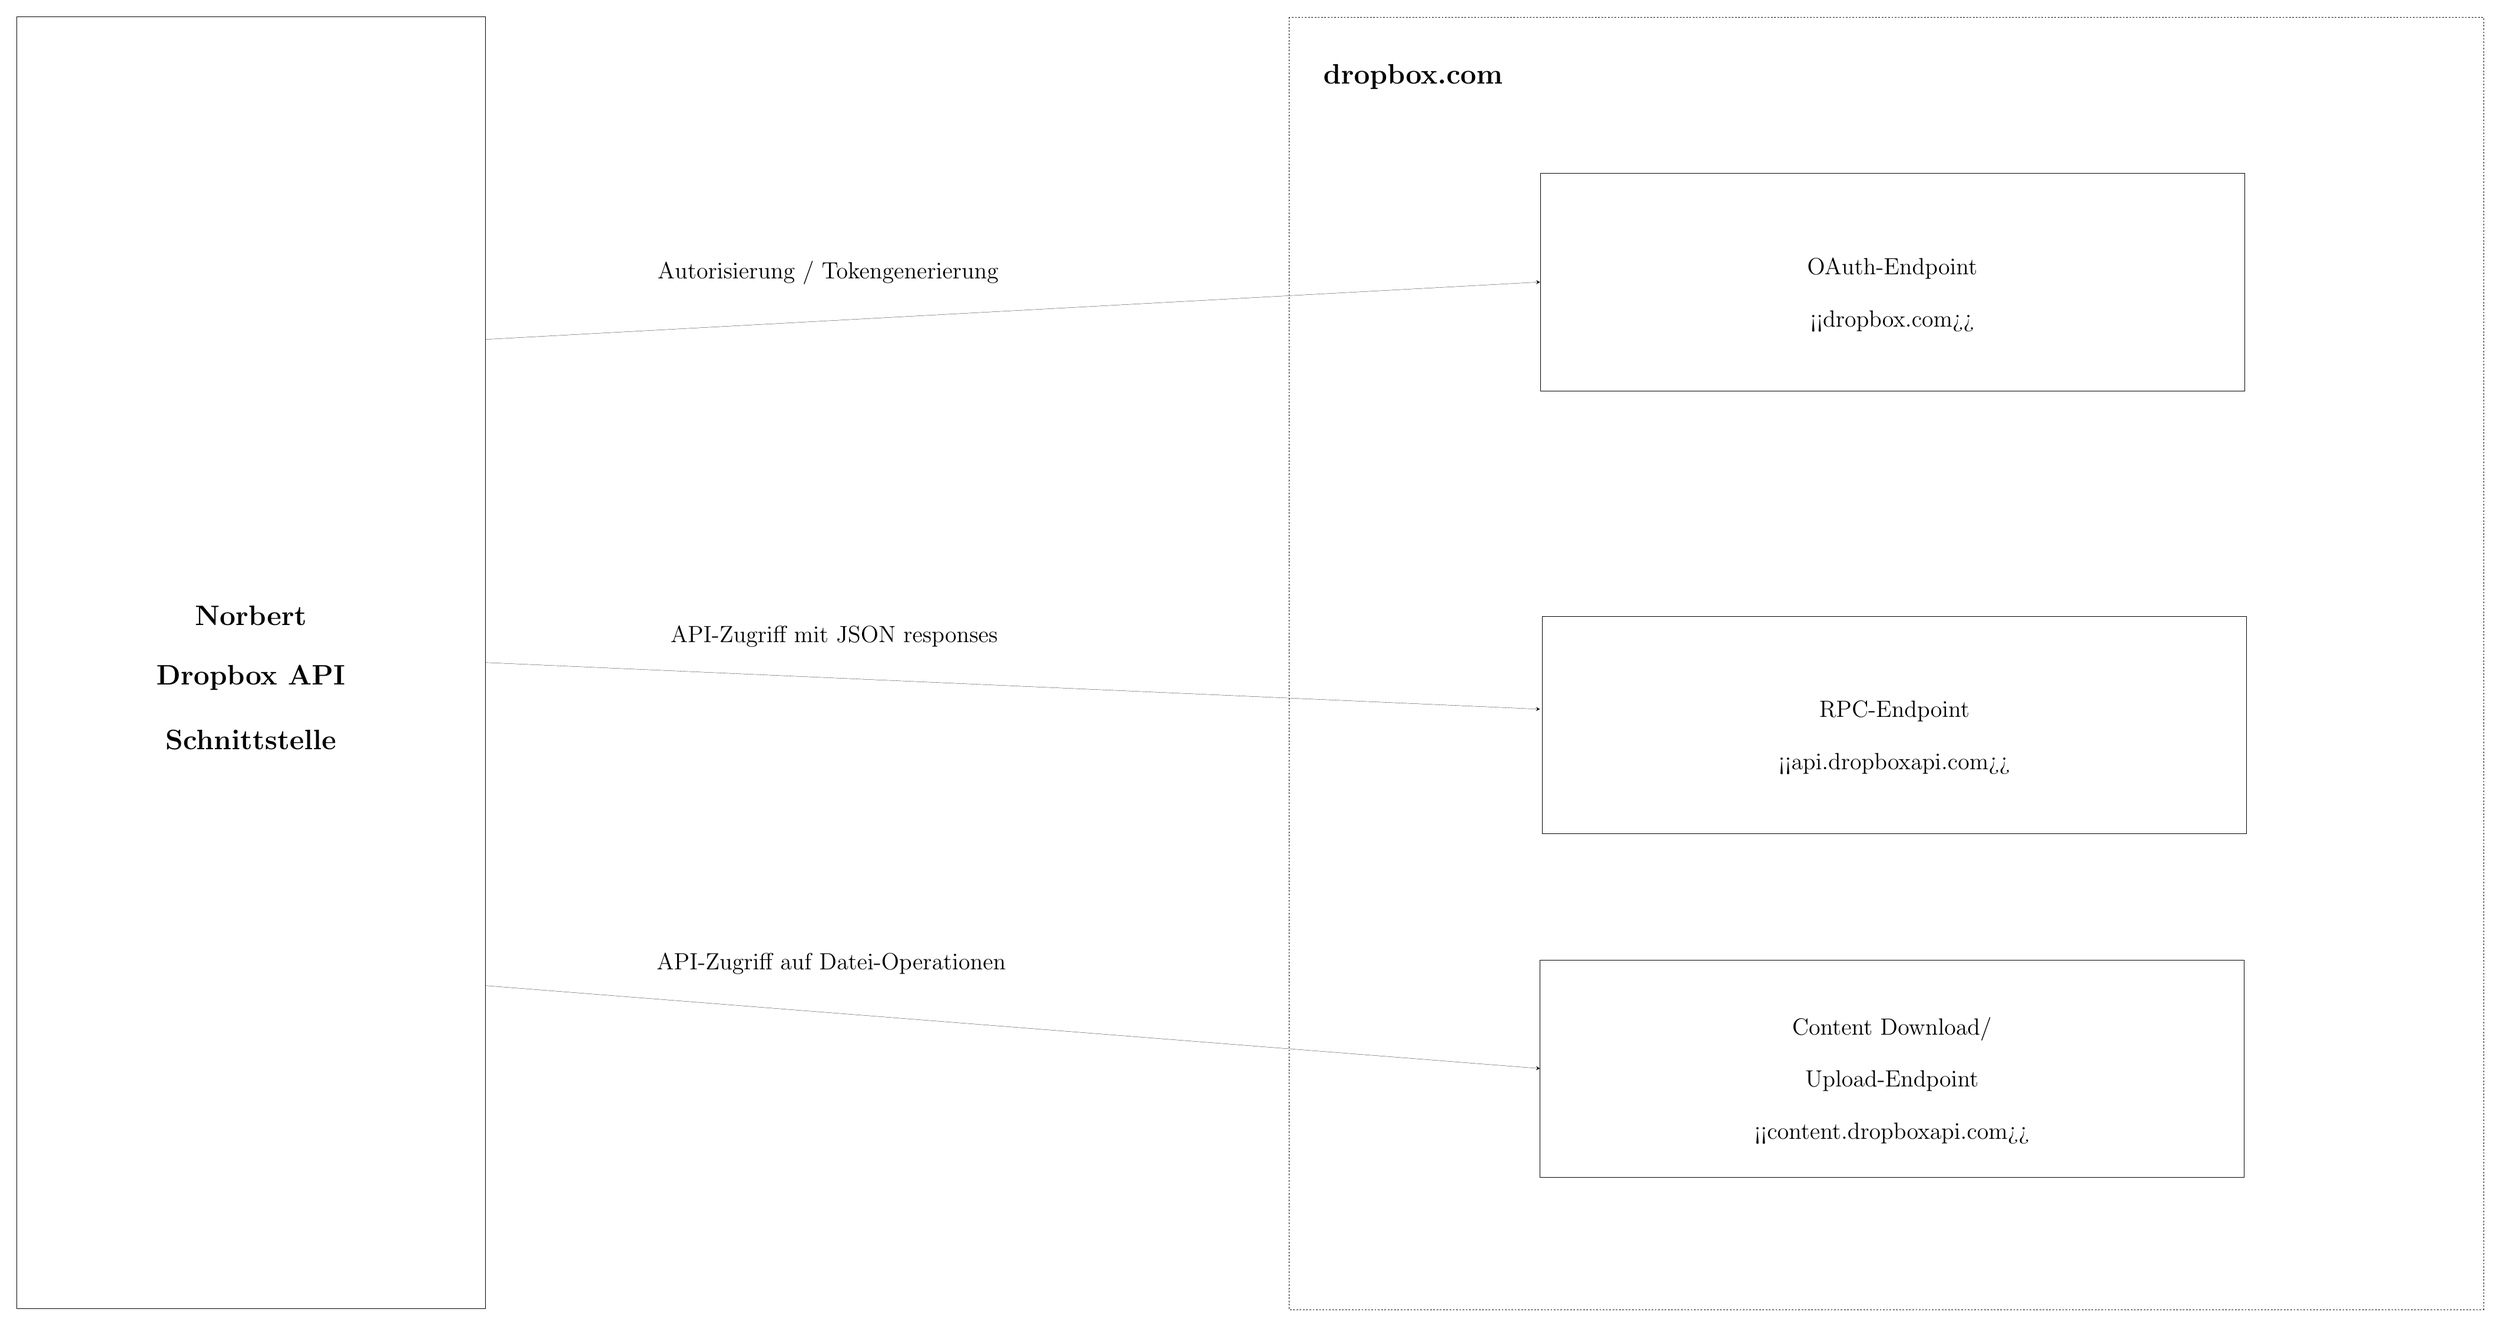
\begin{tikzpicture}
\pgftransformxscale{1.000000}
\pgftransformyscale{-1.000000}
\definecolor{dialinecolor}{rgb}{0.000000, 0.000000, 0.000000}
\pgfsetstrokecolor{dialinecolor}
\definecolor{dialinecolor}{rgb}{1.000000, 1.000000, 1.000000}
\pgfsetfillcolor{dialinecolor}
\definecolor{dialinecolor}{rgb}{1.000000, 1.000000, 1.000000}
\pgfsetfillcolor{dialinecolor}
\fill (8.119868\du,6.074845\du)--(8.119868\du,33.960593\du)--(18.231497\du,33.960593\du)--(18.231497\du,6.074845\du)--cycle;
\pgfsetlinewidth{0.100000\du}
\pgfsetdash{}{0pt}
\pgfsetdash{}{0pt}
\pgfsetmiterjoin
\definecolor{dialinecolor}{rgb}{0.000000, 0.000000, 0.000000}
\pgfsetstrokecolor{dialinecolor}
\draw (8.119868\du,6.074845\du)--(8.119868\du,33.960593\du)--(18.231497\du,33.960593\du)--(18.231497\du,6.074845\du)--cycle;
% setfont left to latex
\definecolor{dialinecolor}{rgb}{0.000000, 0.000000, 0.000000}
\pgfsetstrokecolor{dialinecolor}
\node at (13.175682\du,19.001886\du){\LARGE \textbf{Norbert}};
% setfont left to latex
\definecolor{dialinecolor}{rgb}{0.000000, 0.000000, 0.000000}
\pgfsetstrokecolor{dialinecolor}
\node at (13.175682\du,20.342441\du){\LARGE \textbf{Dropbox API}};
% setfont left to latex
\definecolor{dialinecolor}{rgb}{0.000000, 0.000000, 0.000000}
\pgfsetstrokecolor{dialinecolor}
\node at (13.175682\du,21.682997\du){\LARGE \textbf{Schnittstelle}};
\definecolor{dialinecolor}{rgb}{1.000000, 1.000000, 1.000000}
\pgfsetfillcolor{dialinecolor}
\fill (35.569294\du,6.091693\du)--(35.569294\du,33.977441\du)--(61.330075\du,33.977441\du)--(61.330075\du,6.091693\du)--cycle;
\pgfsetlinewidth{0.100000\du}
\pgfsetdash{{1.000000\du}{1.000000\du}}{0\du}
\pgfsetdash{{1.000000\du}{1.000000\du}}{0\du}
\pgfsetmiterjoin
\definecolor{dialinecolor}{rgb}{0.000000, 0.000000, 0.000000}
\pgfsetstrokecolor{dialinecolor}
\draw (35.569294\du,6.091693\du)--(35.569294\du,33.977441\du)--(61.330075\du,33.977441\du)--(61.330075\du,6.091693\du)--cycle;
% setfont left to latex
\definecolor{dialinecolor}{rgb}{0.000000, 0.000000, 0.000000}
\pgfsetstrokecolor{dialinecolor}
\node at (48.449684\du,20.359289\du){};
% setfont left to latex
\definecolor{dialinecolor}{rgb}{0.000000, 0.000000, 0.000000}
\pgfsetstrokecolor{dialinecolor}
\node[anchor=west] at (48.449684\du,20.034567\du){};
% setfont left to latex
\definecolor{dialinecolor}{rgb}{0.000000, 0.000000, 0.000000}
\pgfsetstrokecolor{dialinecolor}
\node[anchor=west] at (36.193925\du,7.383944\du){\LARGE \textbf{dropbox.com}};
\definecolor{dialinecolor}{rgb}{1.000000, 1.000000, 1.000000}
\pgfsetfillcolor{dialinecolor}
\fill (41.032543\du,19.016385\du)--(41.032543\du,23.709017\du)--(56.222793\du,23.709017\du)--(56.222793\du,19.016385\du)--cycle;
\pgfsetlinewidth{0.100000\du}
\pgfsetdash{}{0pt}
\pgfsetdash{}{0pt}
\pgfsetmiterjoin
\definecolor{dialinecolor}{rgb}{0.000000, 0.000000, 0.000000}
\pgfsetstrokecolor{dialinecolor}
\draw (41.032543\du,19.016385\du)--(41.032543\du,23.709017\du)--(56.222793\du,23.709017\du)--(56.222793\du,19.016385\du)--cycle;
% setfont left to latex
\definecolor{dialinecolor}{rgb}{0.000000, 0.000000, 0.000000}
\pgfsetstrokecolor{dialinecolor}
\node at (48.627668\du,21.071312\du){\Large RPC-Endpoint};
% setfont left to latex
\definecolor{dialinecolor}{rgb}{0.000000, 0.000000, 0.000000}
\pgfsetstrokecolor{dialinecolor}
\node at (48.627668\du,22.200201\du){\Large <<api.dropboxapi.com>>};
% setfont left to latex
\definecolor{dialinecolor}{rgb}{0.000000, 0.000000, 0.000000}
\pgfsetstrokecolor{dialinecolor}
\node[anchor=west] at (49.690330\du,18.401183\du){};
\definecolor{dialinecolor}{rgb}{1.000000, 1.000000, 1.000000}
\pgfsetfillcolor{dialinecolor}
\fill (40.983369\du,26.431875\du)--(40.983369\du,31.124507\du)--(56.165869\du,31.124507\du)--(56.165869\du,26.431875\du)--cycle;
\pgfsetlinewidth{0.100000\du}
\pgfsetdash{}{0pt}
\pgfsetdash{}{0pt}
\pgfsetmiterjoin
\definecolor{dialinecolor}{rgb}{0.000000, 0.000000, 0.000000}
\pgfsetstrokecolor{dialinecolor}
\draw (40.983369\du,26.431875\du)--(40.983369\du,31.124507\du)--(56.165869\du,31.124507\du)--(56.165869\du,26.431875\du)--cycle;
% setfont left to latex
\definecolor{dialinecolor}{rgb}{0.000000, 0.000000, 0.000000}
\pgfsetstrokecolor{dialinecolor}
\node at (48.574619\du,27.922357\du){\Large Content Download/};
% setfont left to latex
\definecolor{dialinecolor}{rgb}{0.000000, 0.000000, 0.000000}
\pgfsetstrokecolor{dialinecolor}
\node at (48.574619\du,29.051246\du){\Large Upload-Endpoint};
% setfont left to latex
\definecolor{dialinecolor}{rgb}{0.000000, 0.000000, 0.000000}
\pgfsetstrokecolor{dialinecolor}
\node at (48.574619\du,30.180135\du){\Large <<content.dropboxapi.com>>};
\definecolor{dialinecolor}{rgb}{1.000000, 1.000000, 1.000000}
\pgfsetfillcolor{dialinecolor}
\fill (40.986152\du,9.460898\du)--(40.986152\du,14.153530\du)--(56.176402\du,14.153530\du)--(56.176402\du,9.460898\du)--cycle;
\pgfsetlinewidth{0.100000\du}
\pgfsetdash{}{0pt}
\pgfsetdash{}{0pt}
\pgfsetmiterjoin
\definecolor{dialinecolor}{rgb}{0.000000, 0.000000, 0.000000}
\pgfsetstrokecolor{dialinecolor}
\draw (40.986152\du,9.460898\du)--(40.986152\du,14.153530\du)--(56.176402\du,14.153530\du)--(56.176402\du,9.460898\du)--cycle;
% setfont left to latex
\definecolor{dialinecolor}{rgb}{0.000000, 0.000000, 0.000000}
\pgfsetstrokecolor{dialinecolor}
\node at (48.581277\du,11.515825\du){\Large OAuth-Endpoint};
% setfont left to latex
\definecolor{dialinecolor}{rgb}{0.000000, 0.000000, 0.000000}
\pgfsetstrokecolor{dialinecolor}
\node at (48.581277\du,12.644714\du){\Large <<dropbox.com>>};
\pgfsetlinewidth{0.100000\du}
\pgfsetdash{}{0pt}
\pgfsetdash{}{0pt}
\pgfsetbuttcap
{
\definecolor{dialinecolor}{rgb}{0.000000, 0.000000, 0.000000}
\pgfsetfillcolor{dialinecolor}
% was here!!!
\pgfsetarrowsend{stealth}
\definecolor{dialinecolor}{rgb}{0.000000, 0.000000, 0.000000}
\pgfsetstrokecolor{dialinecolor}
\draw (18.231497\du,13.046282\du)--(40.986152\du,11.807214\du);
}
% setfont left to latex
\definecolor{dialinecolor}{rgb}{0.000000, 0.000000, 0.000000}
\pgfsetstrokecolor{dialinecolor}
\node[anchor=west] at (21.832636\du,11.607819\du){\Large Autorisierung / Tokengenerierung};
\pgfsetlinewidth{0.100000\du}
\pgfsetdash{}{0pt}
\pgfsetdash{}{0pt}
\pgfsetbuttcap
{
\definecolor{dialinecolor}{rgb}{0.000000, 0.000000, 0.000000}
\pgfsetfillcolor{dialinecolor}
% was here!!!
\pgfsetarrowsend{stealth}
\definecolor{dialinecolor}{rgb}{0.000000, 0.000000, 0.000000}
\pgfsetstrokecolor{dialinecolor}
\draw (18.231497\du,20.017719\du)--(40.983172\du,21.024444\du);
}
% setfont left to latex
\definecolor{dialinecolor}{rgb}{0.000000, 0.000000, 0.000000}
\pgfsetstrokecolor{dialinecolor}
\node[anchor=west] at (22.111685\du,19.457832\du){\Large API-Zugriff mit JSON responses};
\pgfsetlinewidth{0.100000\du}
\pgfsetdash{}{0pt}
\pgfsetdash{}{0pt}
\pgfsetbuttcap
{
\definecolor{dialinecolor}{rgb}{0.000000, 0.000000, 0.000000}
\pgfsetfillcolor{dialinecolor}
% was here!!!
\pgfsetarrowsend{stealth}
\definecolor{dialinecolor}{rgb}{0.000000, 0.000000, 0.000000}
\pgfsetstrokecolor{dialinecolor}
\draw (18.231497\du,26.989156\du)--(40.983369\du,28.778191\du);
}
% setfont left to latex
\definecolor{dialinecolor}{rgb}{0.000000, 0.000000, 0.000000}
\pgfsetstrokecolor{dialinecolor}
\node[anchor=west] at (26.329874\du,19.411982\du){};
% setfont left to latex
\definecolor{dialinecolor}{rgb}{0.000000, 0.000000, 0.000000}
\pgfsetstrokecolor{dialinecolor}
\node[anchor=west] at (21.813661\du,26.521745\du){\Large API-Zugriff auf Datei-Operationen};
\end{tikzpicture}
}
	\caption{API-Zugriffe über die Dropbox-Endpoints}
	\label{04ergebnis:dpendpoints}	
\end{figure}

\section{Webhooks \& Benachrichtigungen}